\chapter{Applications of Convolutional Networks cont.}
% \author{David Brandfonbrener, Min Jae Song, Yuxiao Xie}
% \Lecture date {3/11/19}

\section{Medical Imaging}
CNNs have also been successfully applied to medical imaging. Some examples are:
\begin{itemize}
    \item Brain Tumor Segmentation \cite{braintumor2018}
    \item Skin Cancer Detection \cite{Esteva2017DermatologistlevelCO}
    \item Proximal Femur Segmentation from MR Images \cite{Deniz2018SegmentationOT}
\end{itemize}

However, medical imaging is challenging because of the lack of labeled data.

\subsection{ConvNets in Connectomics}
Connectomics is the study of reconstructing schematics of the brain. Researchers typically proceed by taking a stack of images (thin slices) to get information for the complete volume. One approach to making a 3D reconstruction from 2D images is, of course, using ConvNets \cite{jain2010}. One challenge of this reconstruction is that the neurons are very densely packed and each shape of the neuron is a strong indicator of its role. Hence, the reconstructions have to be very accurate and high-res.

\subsection{3D ConvNets for Medical Image Analysis}

\subsubsection{U-Net}
\begin{figure}[ht]
    \centering
    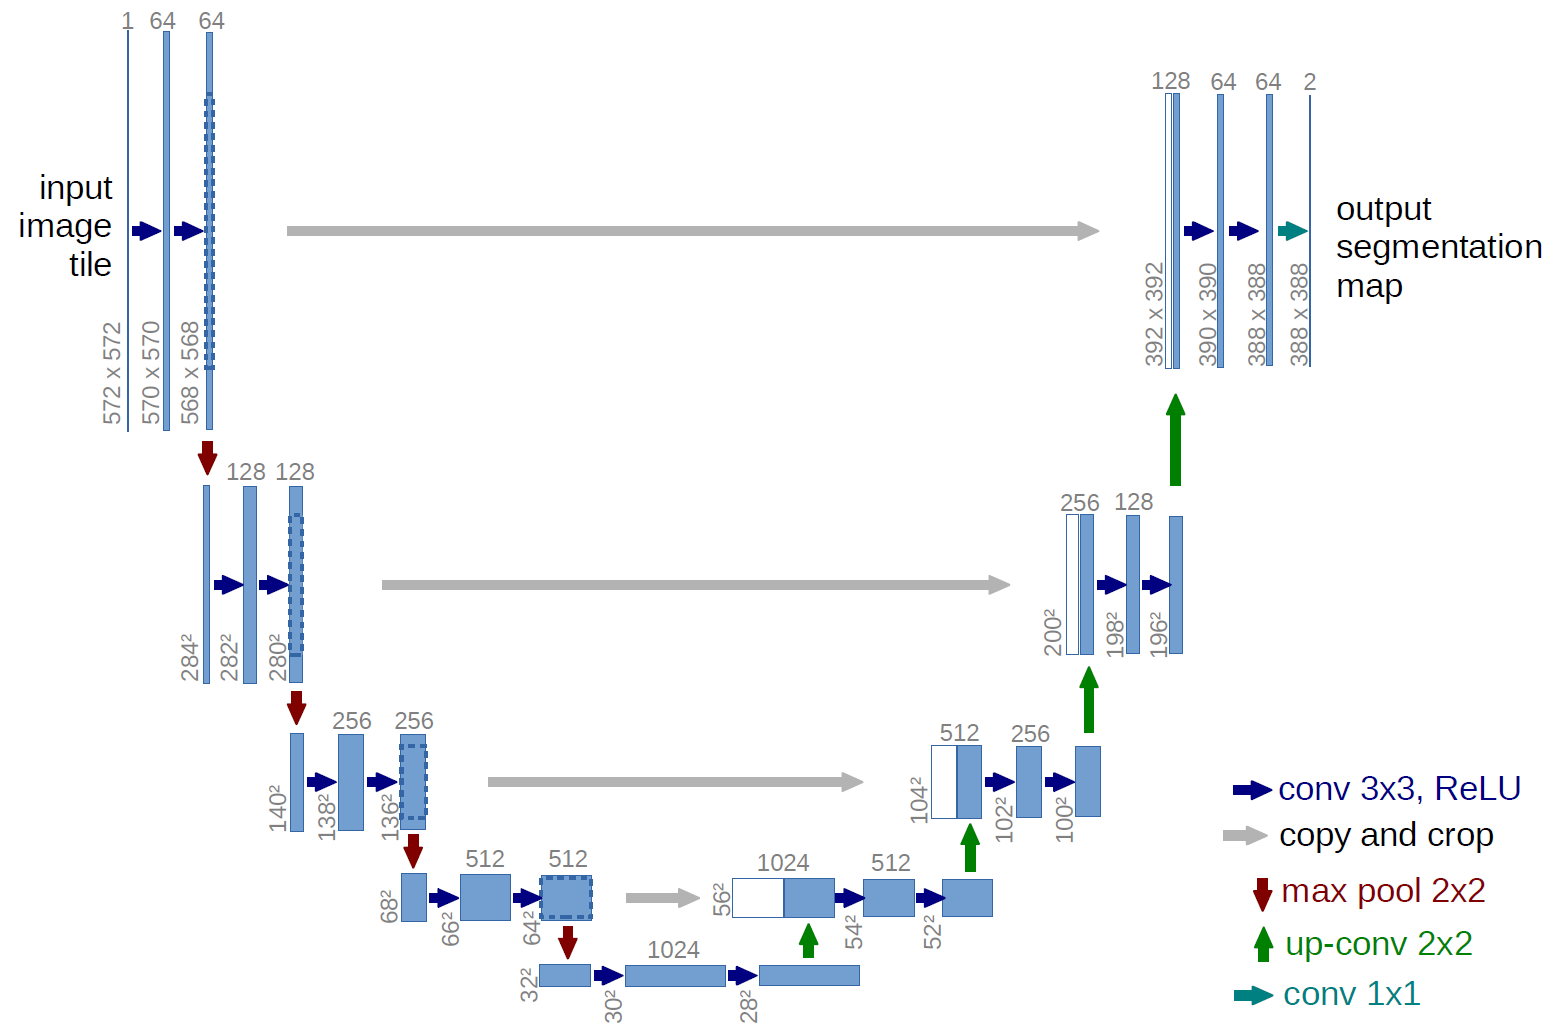
\includegraphics[width=0.75\textwidth]{lectures/06-a/unet.png}
    \caption{U-net architecture from \citep{unet}}
    \label{fig:unet}
\end{figure}

In medical imaging applications, the U-Net architecture is often used. This architecture consists of a cascade of convolutional filters that downsample the input image from high-resolution to low resolution as in a normal ConvNet and then a series of "deconvolution" filters that upsample the representation back to high resolution (along with skip connections across the "U" structure to make up for the loss of resolution during the downsampling phase). Figure \ref{fig:unet} shows the U-Net architecture. U-Net has won the EM segmentation challenge at ISBI 2012 by a large margin.

\begin{figure}[ht]
    \centering
    \begin{subfigure}{0.25\textwidth}
    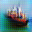
\includegraphics[width=0.9\linewidth]{lectures/06-a/checkerboard0.png} 
    \end{subfigure}
    \begin{subfigure}{0.25\textwidth}
    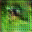
\includegraphics[width=0.9\linewidth]{lectures/06-a/checkerboard1.png}
    \end{subfigure}
    \begin{subfigure}{0.25\textwidth}
    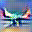
\includegraphics[width=0.9\linewidth]{lectures/06-a/checkerboard2.png}
    \end{subfigure}
    \caption{checkerboard artifacts from \citep{odena2016deconvolution}}
    \label{fig:checkerboard}
\end{figure}

However, one issue with deconvolution is that it can produce "checkerboard" artifacts because of uneven overlaps. Deconvolution is essentially a convolution in reverse, except the pooling step now is replaced with upsampling. There are several different ways to do this upsampling. One naive choice is just repeating the same value over all pixels in the upsampled region, which can lead to aforementioned checkerboard artifacts. Another choice is bilinear interpolation between nearby pixels at the lower resolution to get smoother upsampled image. A third way is a switch type upsampling that tries to mimic an inverse to max-pooling. This can be implemented by remembering the pixel position selected by max pooing during the downsampling step and, in the upsampling step, copying the low-res pixel to the corresponding upsampled pixel position and filling in other pixels with 0's.
\section{Point Cloud Data}
Some 3D data can be represented as 2D images along with estimates of the depth of each pixel. This depth estimate comes from either stereo cameras or LIDAR systems. Unfortunately, the LIDAR is very expensive and often unreliable (eg. doesn't work well when it rains) so some applications like self-driving cars are trying to find other ways to estimate depth.

Point cloud (Figure \ref{fig:pointcloud}) is another way of representing 3D data. The data here consists of a "cloud" of $(x,y,z)$  coordinates along with RGB values. However, point clouds are very sparse since most voxels do not contain any object. This causes problems for traditional ConvNets because the input would be almost entirely zeros.

\begin{figure}[ht]
    \centering
    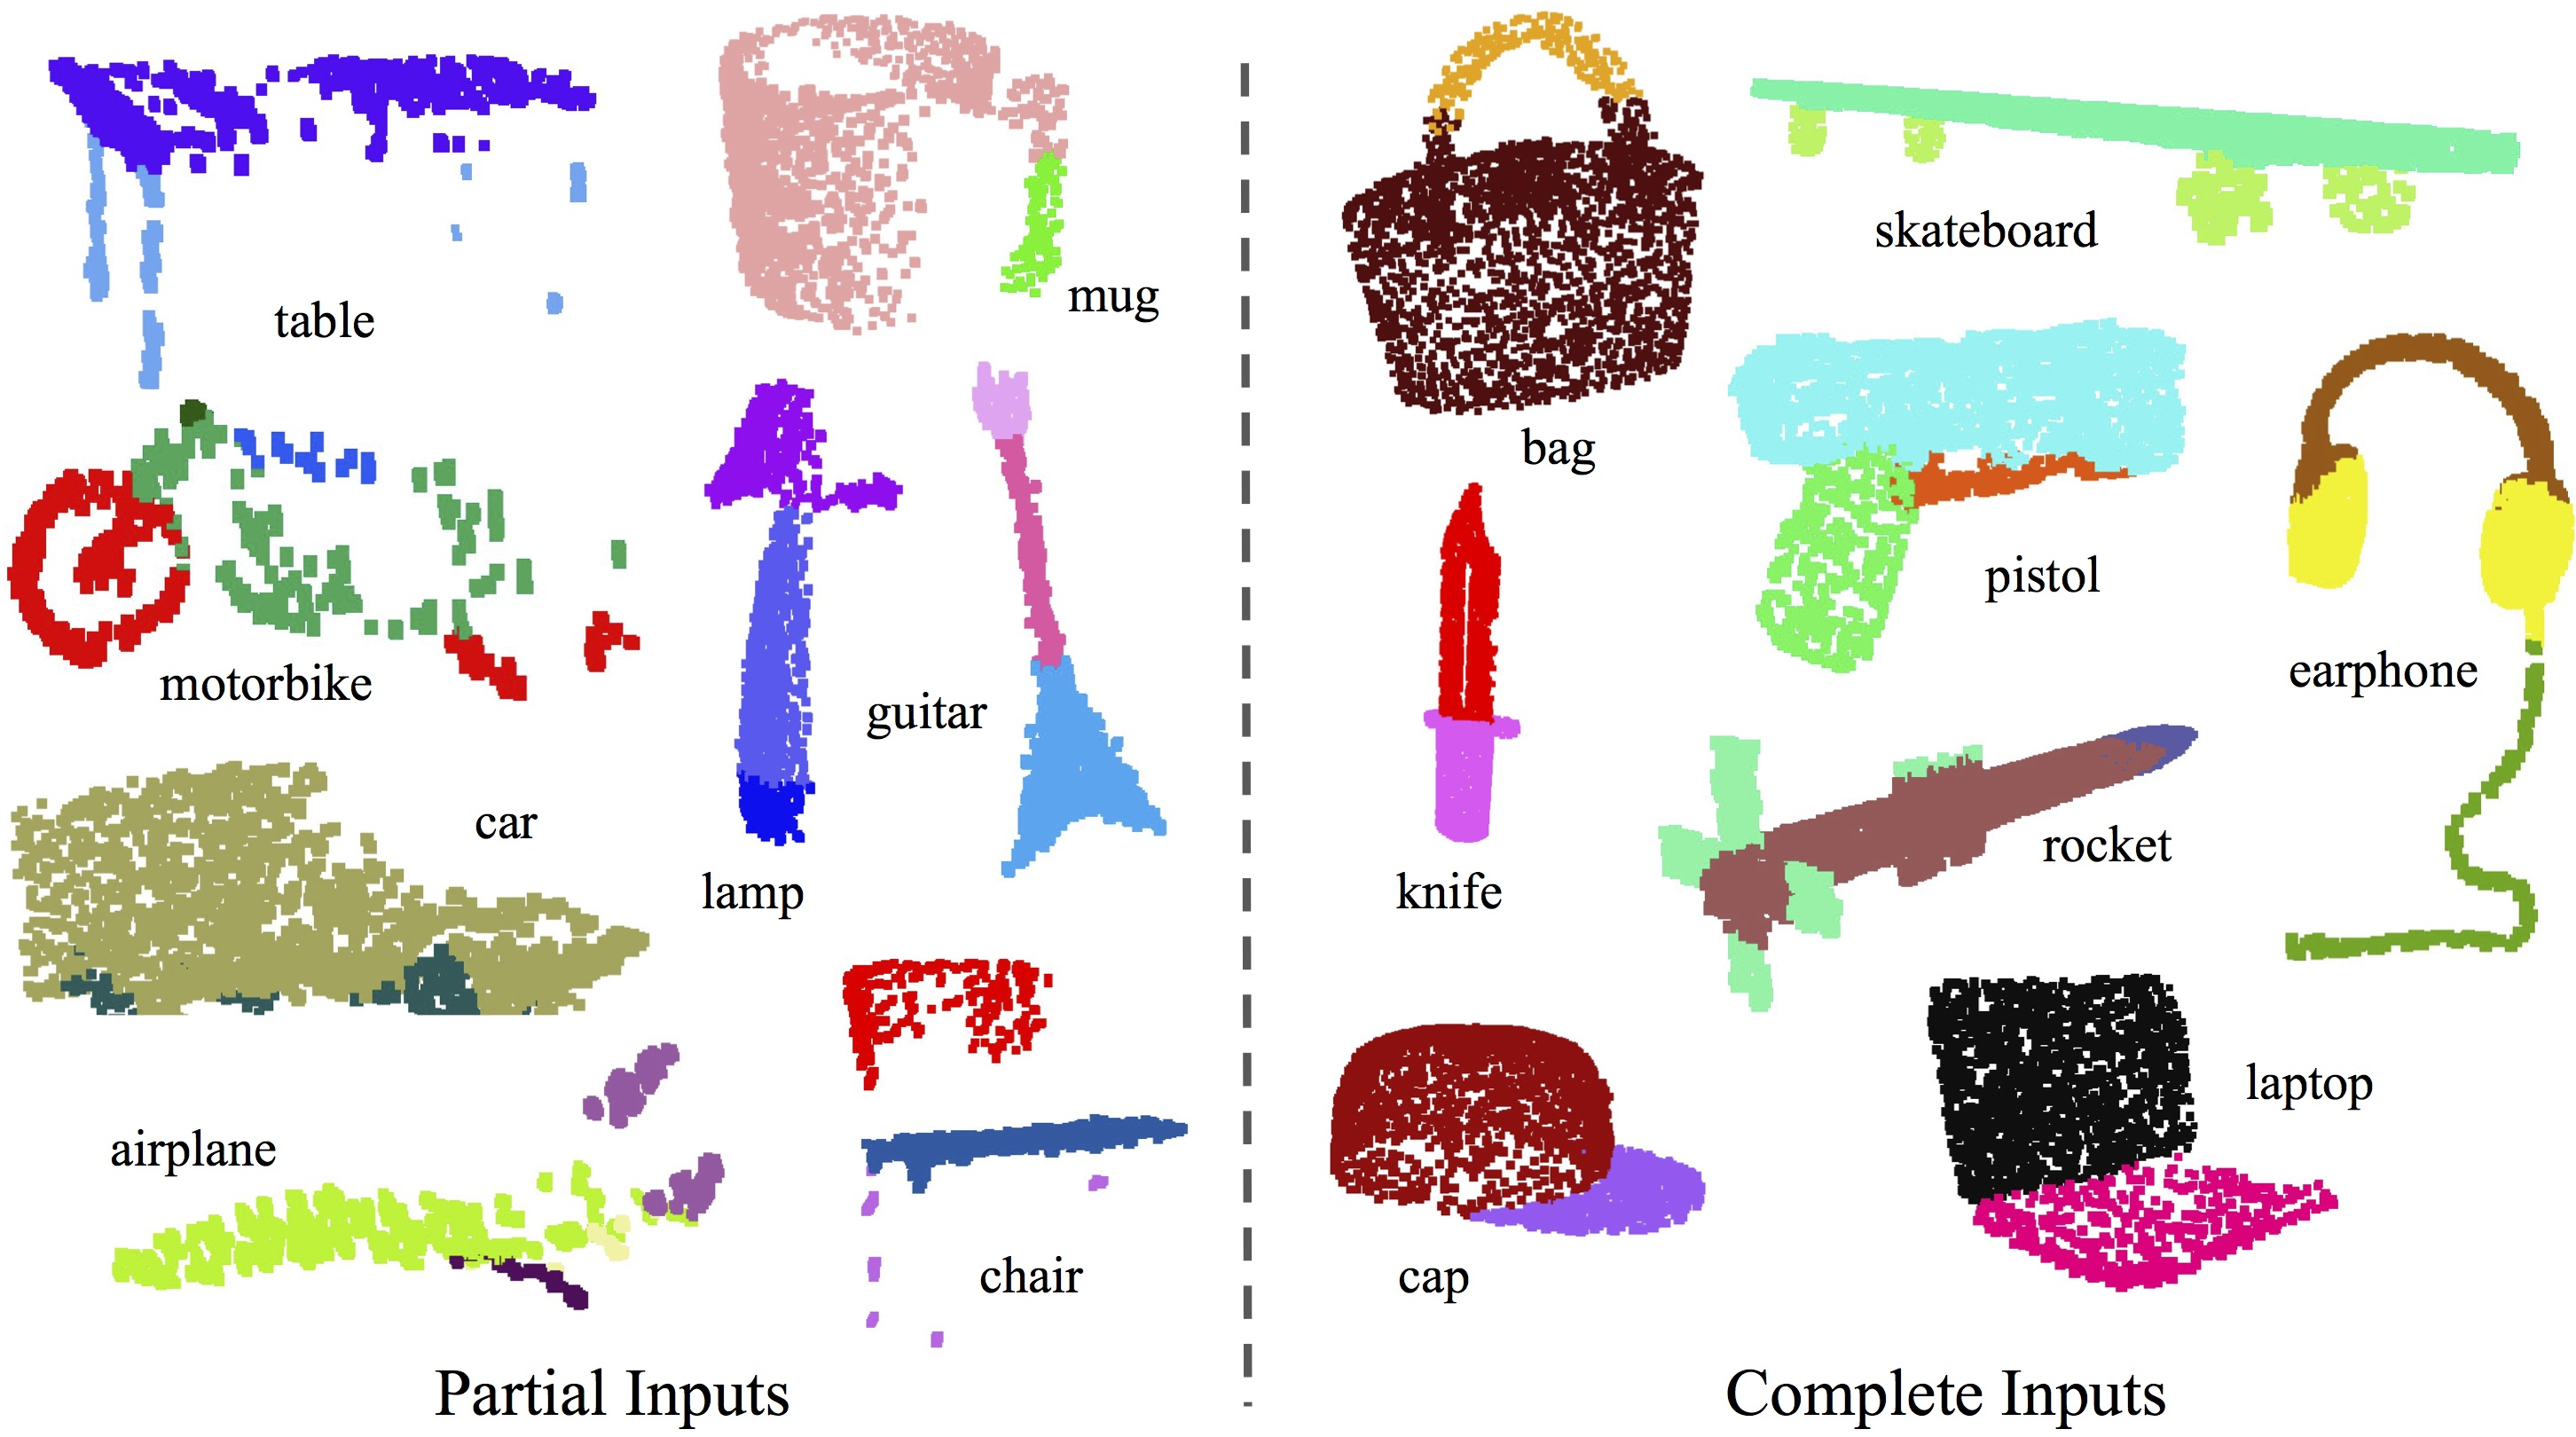
\includegraphics[width=0.75\textwidth]{lectures/06-a/pointnet.jpg}
    \caption{Point cloud images from \citep{qi2017pointnet}}
    \label{fig:pointcloud}
\end{figure}
Different variants of ConvNets have been invented to work with this kind of data. For example, there was a ShapeNet competition on semantic segmentation of 3D point cloud data.
The winner was the "Submanifold Sparse ConvNet". This method implements {\it sparse convolutions} that efficiently operate on sparse data. If we use normal convolutions on sparse inputs, then a lot of the computation is wasted since we would be multiplying zeros most of the time. The {\it sparse convolutions} introduced in this work prevent this waste by keeping track of which "sites" contain information (via a hash table) and not performing convolutional operations on those sites. Another alternative is the various variants of graph CNNs which extend ConvNets to data with non-gridlike structure.

\section{Speech Recognition}
ConvNets can also be used on audio data. To feed audio data to a ConvNet, we can use spectrograms or cepstrograms, which are 2-dimensional plots that show changes in the frequency component of the audio signal with respect to time.

There are mainly two approaches to speech recognition:
\begin{enumerate}
    \item Classical approach: First train an HMM/GMM model to align the phones with the audio signal, and then train the model to map audio signals to these aligned phones.
    \item End-to-end approach (Wav2Letter): The model goes from speech signal to letter transcription directly without intermediate phonetic transcriptions. The input data can be either a spectrogram or even raw waveform \cite{Collobert2017Wav2LetterAE}.
\end{enumerate}
The aim of an Automatic Speech Recognition(ASR) system is to find the most likely sentence (word sequence) $W$ which transcribes the speech audio $A$, with acoustic model $P(A|W)$ and language model $P(W)$. The general process of utilizing ConvNets for speech recognition can be illustrated as Figure \ref{fig:cnn_asr}.
Useful techniques for speech feature extraction are Short-time Fourier Transforms(STFTS), Mel-frequency cepstrum (MFFCs), Linear Predictive Coding (LPC), etc (\ref{fig:feature}). Then a ConvNet is trained on labeled transcriptions for frame-level classification. Further alighment techniques such as Hidden Markov Models will be applied to get phones. Then the alighed phones will be fit into some pre-trained lexicon model to get the corresponding words. At last, a language model will be applied to the words to get the transcription. 
\begin{figure}[ht]
    \centering
    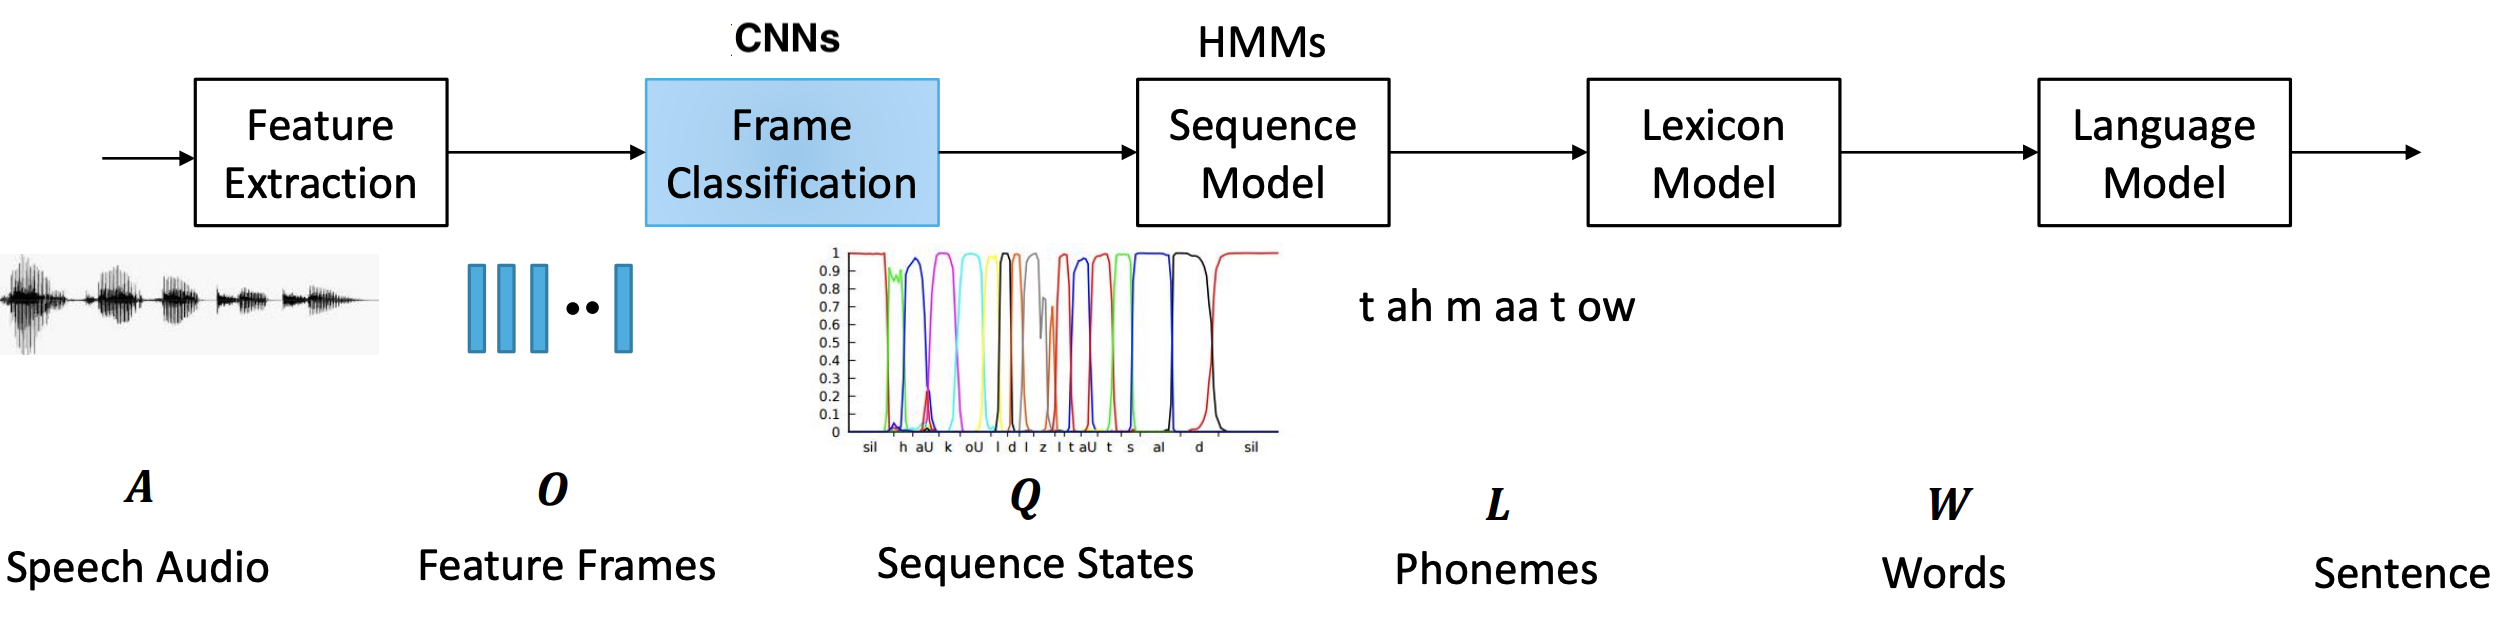
\includegraphics[width=1\textwidth]{lectures/06-a/cnn_asr.png}
    \caption{CNN-HMM ASR system architecture}
    \label{fig:cnn_asr}
\end{figure}
\begin{figure}[ht]
    \centering
    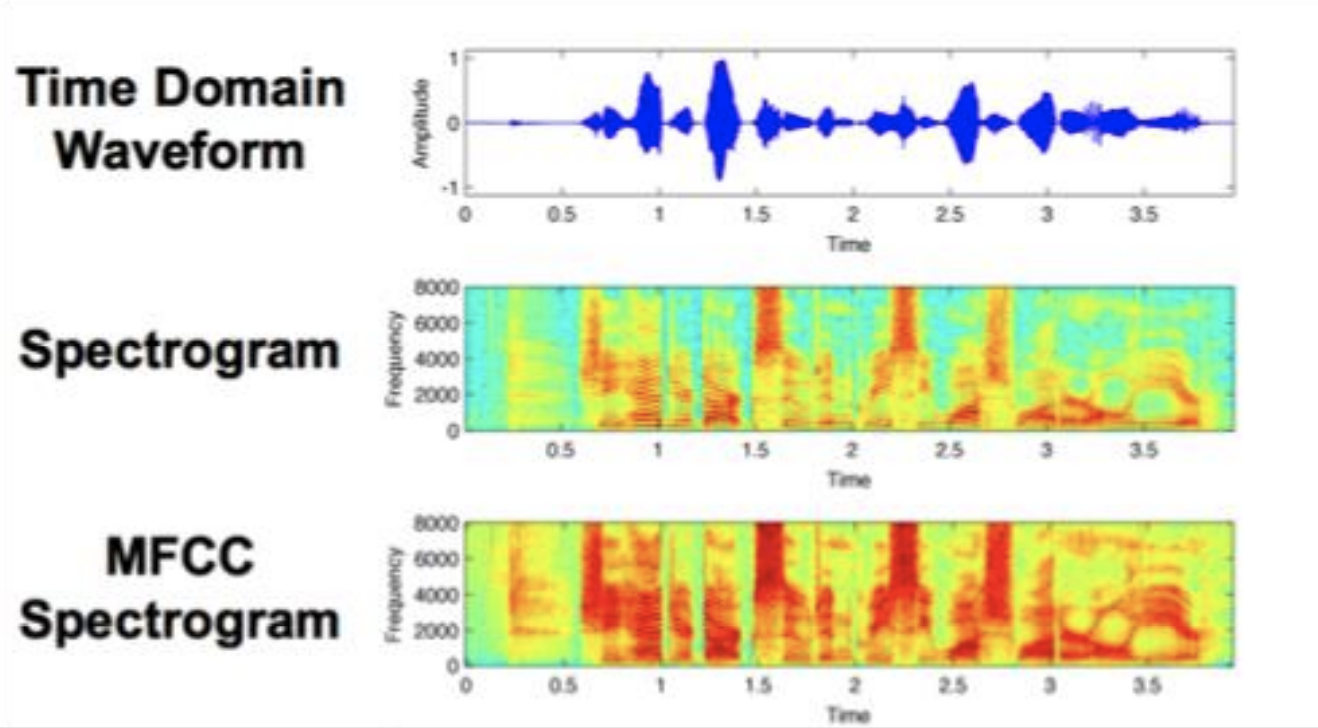
\includegraphics[width=0.75\textwidth]{lectures/06-a/feature.png}
    \caption{speech audio representations}
    \label{fig:feature}
\end{figure}